\section{Superfluïde Æther Framework}

We veronderstellen een stationaire, Euclidische 3-dimensionale æther die zich gedraagt als een superfluïde met een viscositeit van nul en een constante massadichtheid. Dit continue medium vormt de basis van alle natuurkunde: deeltjes zijn topologische wervelstructuren in de æther en velden corresponderen met stromingspatronen (vorticiteit, druk, etc.). De dynamica wordt bepaald door klassieke stromingsvergelijkingen, met de volgende fundamentele postulaten:

\begin{figure}[htbp]
    \centering
    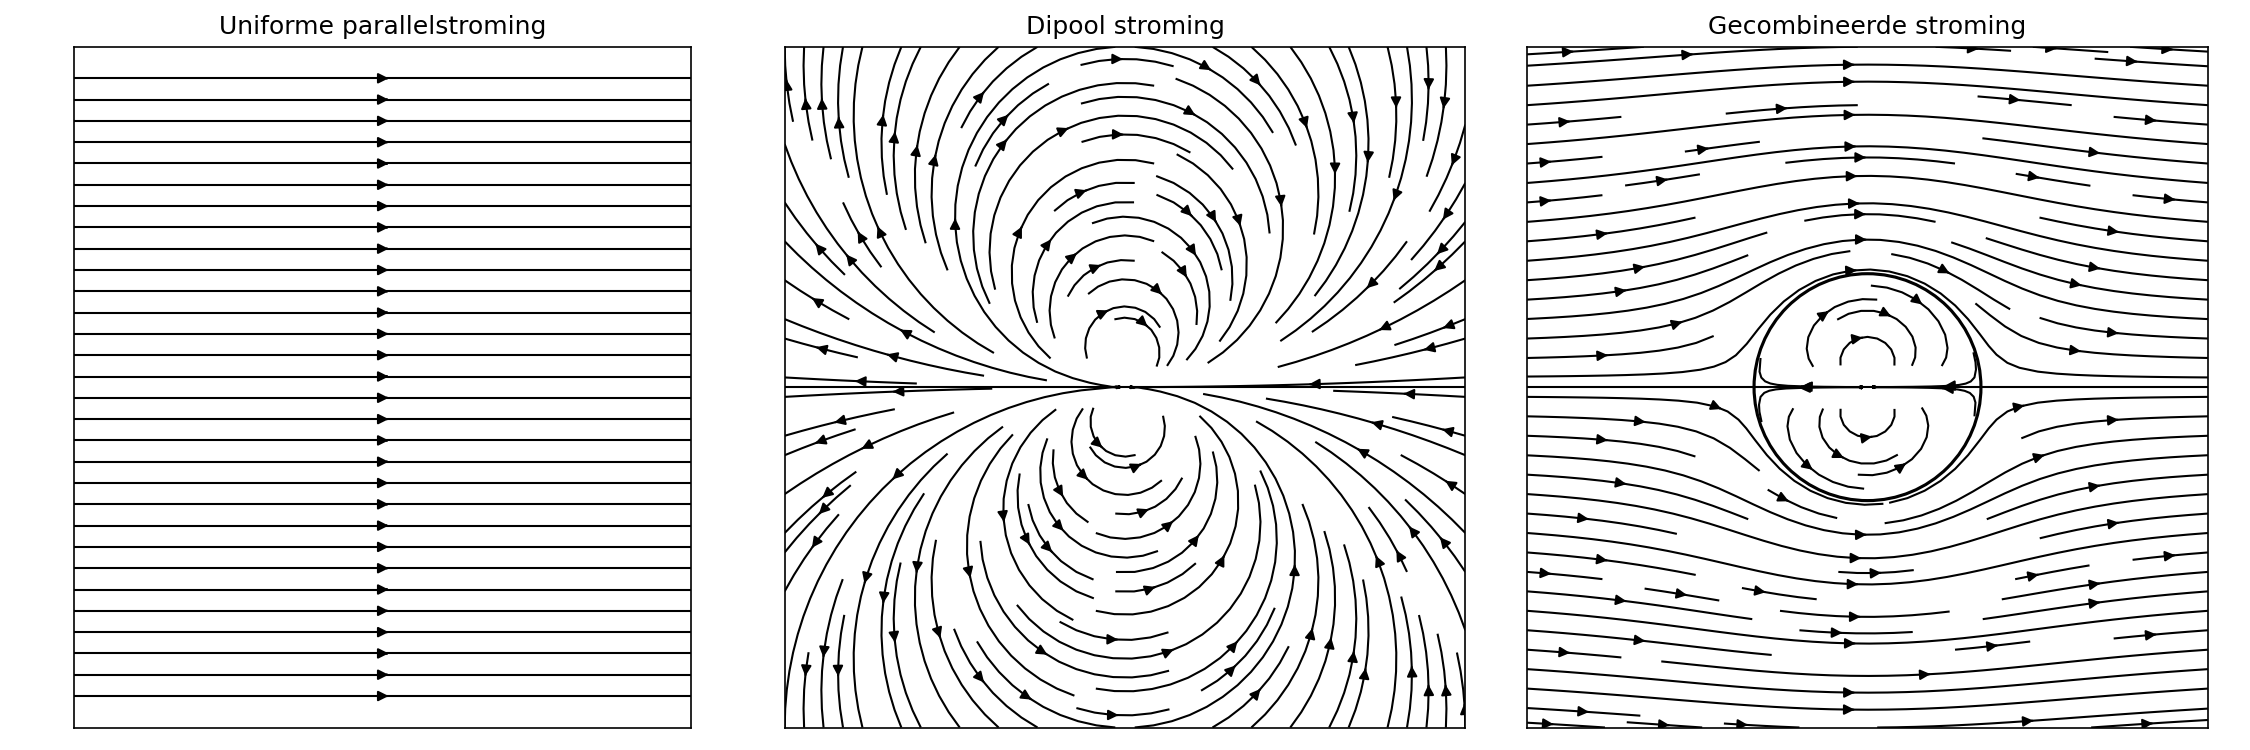
\includegraphics[width=0.85\textwidth]{03-combined_flow}
    \caption{Illustratie van ætherstroming en vorticiteit rond wervelkernen.}
    \label{fig:vortexfields}
\end{figure}
\begin{description}

    \item[\textbf{Postulaat I: Absolute vlakke ruimte}] \hfill \\
    Ruimte is een stationaire, vlakke Euclidische achtergrond met een voorkeursframe gedefinieerd door de æther in rust. Alle afstanden en snelheden worden hierin gemeten. Er is geen intrinsieke ruimtetijdkromming; alle metrieken zijn afgeleid uit stromingsvelden. (Dit is vergelijkbaar met Lorentz's oorspronkelijke absolute frameconcept, maar nu met een fysieke superfluïde die de ruimte vult~\cite{Winterberg2002-PlanckAether}).

    \item[\textbf{Postulaat II: Onsamendrukbaar uniforme æther}] \hfill \\
    De æther is een ideale vloeistof met constante dichtheid $\rho_{\ae}$, nul viscositeit, en nul samendrukbaarheid (analoog aan supervloeibaar helium bij $T=0$). Daarom kunnen æthervolume-elementen niet worden gecreëerd of vernietigd; Stroming is divergentieloos, behalve mogelijk bij singuliere wervelkernen.  Alle lokale variaties (bijv. nabij massa's) hebben betrekking op snelheidsvelden of druk, niet op dichtheidsveranderingen.

    \item[\textbf{Postulaat III: Wervelknopen als materie}] \hfill \\
    Materiedeeltjes worden gemodelleerd als stabiele, topologisch geconserveerde wervelknopen. Volgens Kelvin~\cite{Kelvin1867-vortex} is een atoom of fundamenteel deeltje een gekwantiseerde wervellus of -knoop in de æther. Het heeft een goed gedefinieerde kern (van de orde van de Planck-lengte $l_{\textrm P}$ in straal, volgens de Planck-æther-theorieën~\cite{Winterberg2002-PlanckAether}) waar æther circulair omheen stroomt. De topologie van de wervel (knooptype) zou kunnen overeenkomen met het type deeltje, terwijl de intrinsieke hoeksnelheid $\omega$ (de wervelsnelheid van æther rond de kern) het deeltje zijn interne klok geeft.

    \item[\textbf{Postulaat IV: Tijd als kernrotatie}] \hfill \\
    De juiste tijd voor een deeltje wordt gedefinieerd door de rotatie van zijn wervelkern. Bijvoorbeeld, een bepaalde vaste rotatiehoek (zeg één volledige $2\pi$ omwenteling van de kern) zou een vaste hoeveelheid juiste tijd kunnen definiëren (misschien in de orde van één \("\)tik\("\)). De leeftijd of interne tijd van een deeltje gaat vooruit met het aantal omwentelingen dat zijn kern uitvoert. Snellere kernrotatie betekent een snellere interne tijdssnelheid. Belangrijk is dat deze rotatie een absoluut fysiek proces is dat plaatsvindt ten opzichte van de æther.

    \item[\textbf{Postulaat V: Thermodynamiek als emergent gedrag}] \hfill \\
    Temperatuur, entropie en thermische fluctuaties ontstaan statistisch uit microscopische ætherstroming. Fundamenteel is het medium echter niet-thermisch en perfect dissipatieloos. In het grootste deel van de æther (ver van wervelkernen) kan de stroming irrotationeel en laminair zijn. Macroscopische thermodynamische concepten (temperatuur, entropie) worden statistisch gezien verondersteld voort te komen uit kleinschalige ætherdynamica, maar op fundamenteel niveau is de æther een dissipatieloos, niet-thermisch medium. Daarom negeren we alle eindige-temperatuur- of viskeuze effecten – de æther is een perfecte niet-viskeuze vloeistof. Alleen wervelinteracties en drukvelden spelen een rol.

    \item[\textbf{Postulaat VI: Krachten via vorticiteit}] \hfill \\
    Alle krachten (elektromagnetisme, zwaartekracht, enz.) worden gemedieerd door ætherstromen.
    Ruimtelijke gradiënten in vorticiteit of heliciteit (draaiing van wervellijnen) in het ætherveld kunnen andere vortices beïnvloeden. Bijvoorbeeld, wat wij waarnemen als een $\text{"zwaartekrachtsveld"}$ zal worden gemodelleerd door een bepaald æthersnelheidsveld (zoals we later zullen toelichten). Het principe van maximale kracht $ F_\text{max} = c^4 / 4 G $ uit de algemene relativiteitstheorie~\cite{Schiller2022-maxforce}, dat een bovengrens stelt aan kracht in de natuur, wordt verondersteld voort te komen uit de eigenschappen van de æther (bijv. maximale stroomsnelheid $c$ en dichtheid $\rho_\text{\ae}$ leggen een limiet op aan impulsflux/kracht).
\end{description}



Binnen dit raamwerk biedt de æther een absolute referentie voor beweging, maar alle meetbare effecten moeten uiteindelijk consistent zijn met de relativiteitstheorie. Zoals Winterberg (2002) het formuleerde, ``kan het universum worden beschouwd als Euclidische vlakke ruimtetijd, op voorwaarde dat we een dichtbevolkt kwantumvacuüm superfluïde als æther opnemen''~\cite{Winterberg2002-PlanckAether}.


\begin{figure}[htbp]
    \centering
    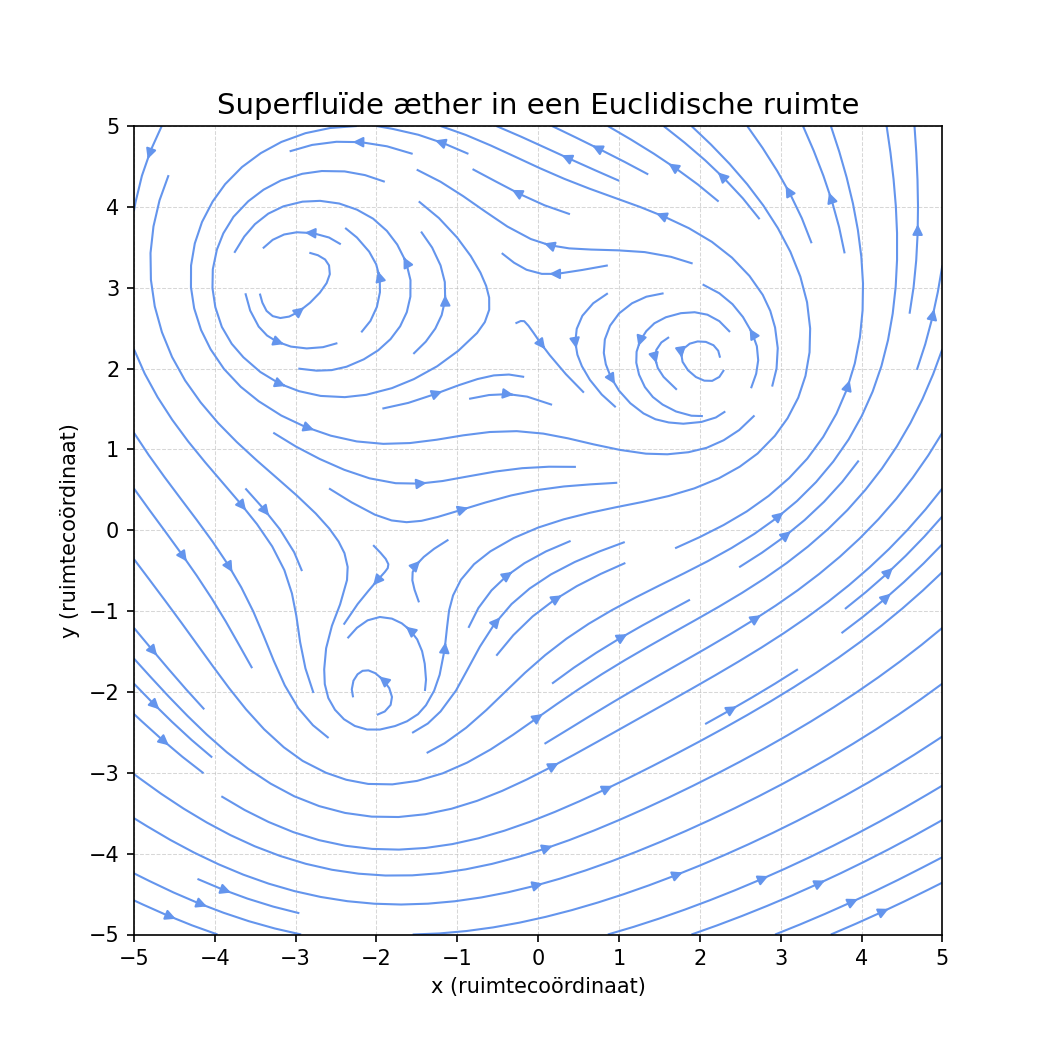
\includegraphics[width=0.85\textwidth]{04-ÆtherSuperfluïde}
    \caption{Uniforme ætherstroom met daarin ingebedde wervelstructuren. De æther is voorgesteld als een ideale superfluïde met behoud van vorticiteit.}
    \label{fig:ÆtherSuperfluïde}
\end{figure}


\textbf{Definities en constanten:} Voor later gebruik definiëren we enkele fundamentele constanten in dit model. De Planck-tijd is
\[
    t_{\textrm P} = \sqrt{\frac{\hbar G}{c^5}} \approx 5.39\times10^{-44}\ \text{s},
\]
de natuurlijke eenheid van tijd in kwantumzwaartekracht. Het vertegenwoordigt ongeveer de tijd die licht nodig heeft om één Planck-lengte $l_{\textrm P} \approx 1.62\times10^{-35}$ m af te leggen. In veel superfluïde-æther-theorieën zou $l_{\textrm P}$ de kerndiameter van elementaire wervelstructuren kunnen zijn~\cite{Winterberg2002-PlanckAether}, dus één volledige rotatie van een elementaire wervelstructuur met de lichtsnelheid $c$ zou de orde van $t_{\textrm P}$ aannemen. Dus $t_{\textrm P}$ stelt een bovengrens in voor de rotatiefrequentie ($\sim 10^{43}$ s$^{-1}$) voor elke fysieke klok in de æther.

Een andere nuttige constante is de voorgestelde maximale kracht:

\begin{equation*}
    F_\text{max} = \frac{c^4}{4G} \approx 3.0\times10^{43}\ \text{N}.
\end{equation*}

Dit verschijnt als een bovengrens in de algemene relativiteitstheorie~\cite{Schiller2022-maxforce}, bijvoorbeeld, de zwaartekracht tussen twee zwarte gaten kan $F_\text{max}$ niet overschrijden. In de æther-afbeelding kan $F_\text{max}$ worden geïnterpreteerd als de maximale spanning of sleepkracht die de superfluïde æther kan verdragen wanneer stromingen de lichtsnelheid naderen.

We behouden $c$ (snelheid van het licht in vacuüm) als de karakteristieke signaalsnelheid in de æther (bijv. de snelheid van geluid of golfvoortplanting in het superfluïde vacuüm, vaak genomen als $c = \sqrt{B/\rho_{\text{\ae}}}$ voor bulkmodulus $B$). De Newtoniaanse gravitatieconstante $G$ zal ingaan bij het koppelen van ætherstroming aan massa (aangezien massa in wezen een wervel is met een bepaalde circulatie en kernstructuur die verband houdt met $G$). We zullen indien nodig extra constanten introduceren.